\documentclass[12pt]{amsart}
\usepackage[T1]{fontenc}
\usepackage[margin=1in]{geometry}
\usepackage{amsmath,amssymb,amsthm,booktabs,graphicx}
\usepackage[hidelinks]{hyperref}
\usepackage{microtype}
\newtheorem{proposition}{Proposition}
\newtheorem{corollary}[proposition]{Corollary}
\graphicspath{{../figures/}{figures/}}
\newcommand{\MaximumN}{10}
\newcommand{\MaximumSide}{20}
\newcommand{\RawSixteen}{1517021583328338160591145724550850}
\newcommand{\OrbitSixteen}{189627697916042276889063633686282}
\newcommand{\PeakStates}{677,909}
\newcommand{\RunSeconds}{11.01}
\newcommand{\PeakMemory}{315.8}

\title[Hamiltonian cycles with a central hole]{Hamiltonian cycles on square grids\protect\\with a central $2\times2$ hole}
\author{Jason Roell}

\date{September 26, 2026}
\subjclass[2020]{05C30, 05C45, 05C85}
\keywords{Hamiltonian cycle, grid graph, transfer matrix, integer sequence, dihedral symmetry}

\raggedbottom
\begin{document}
\begin{abstract}
We enumerate undirected Hamiltonian cycles on the $2n\times2n$ lattice grid
with its four central vertices deleted, for $1\leq n\leq\MaximumN$.
Two frontier implementations with different connectivity encodings give
identical exact counts. Half-board and quarter-board reductions count cycles
fixed by square symmetries, yielding geometric orbit counts and exact
stabilizer classes. We prove that quarter-turn symmetry is impossible when
$n$ is odd. A separate edge-orbit search verifies the symmetry counts
through the $8\times8$ case, and additionally verifies quarter-turn and
both-axis counts through $12\times12$. The source code, tables, resource measurements,
and verification procedures are public. The finite-size comparisons are
descriptive and do not establish a new limiting growth constant or exponent.
\end{abstract}
\maketitle

\section{Definition and exact sequence}
Let $G_n$ have vertices $(x,y)$ with $1\leq x,y\leq2n$, except for
$(n,n)$, $(n,n+1)$, $(n+1,n)$, and $(n+1,n+1)$.
Edges join lattice neighbors. For $n\geq2$, the graph has $4n^2-4$ vertices
and $8n^2-4n-12$ edges. Let $H_n$ count its Hamiltonian cycles as undirected
edge sets, with neither a starting vertex nor a direction distinguished.
Rotated and reflected edge sets are initially distinct. Set $H_1=0$,
since $G_1$ is empty. The first nonempty case $G_2$ is a single $12$-cycle.

\begin{table}[htbp]
\centering
\begin{tabular}{rrr}
\toprule
$n$ & $|V(G_n)|$ & $H_n$ \\
\midrule
1 & 0 & 0 \\
2 & 12 & 1 \\
3 & 32 & 14 \\
4 & 60 & 164102 \\
5 & 96 & 9684216390 \\
6 & 140 & 27867828294632440 \\
7 & 192 & 1167509412814480584454378 \\
8 & 252 & 1517021583328338160591145724550850 \\
9 & 320 & 35604867201983888335090959513825934093936960 \\
10 & 396 & 22194400531163887940263507134424320689889325050239815212 \\
\bottomrule
\end{tabular}

\caption{Undirected Hamiltonian cycles on the centrally punctured grid.}
\label{tab:raw}
\end{table}

The computation gives the complete table through $n=\MaximumN$ shown in
Table~\ref{tab:raw}. In particular,
\[
H_8=\RawSixteen.
\]
The number $O_n$ of geometric orbits under the eight symmetries of the square
is calculated in Section~\ref{sec:burnside}. The code and data are at
\begin{center}
\url{https://github.com/jroell/punctured-grid-cycles}.
\end{center}
The counting programs and complete data are fixed at commit
\href{https://github.com/jroell/punctured-grid-cycles/tree/2d0d15baa21d21f9436bcf5736be4969a0ad818f}{\texttt{2d0d15b}}. The revised manuscript and its build instructions
are in the same repository.

Connectivity transfer methods are established techniques for Hamiltonian
grid enumeration. The present calculation adapts them to this central
puncture. The relation to earlier work is discussed in
Section~\ref{sec:reproducibility}.

\section{Frontier recurrence and correctness}
Process lattice positions in row-major order. A frontier separates
processed positions from unprocessed positions and has at most $w+1$ slots
for a board of width $w$. Each slot is empty or carries a selected edge to
the unprocessed side. Every processed vertex has its required degree, and
every component built so far is a path. The state records which occupied
slots are the two ends of each path.

In the primary implementation, planarity makes the endpoint pairing
noncrossing. Empty slots are encoded by $0$, and the two ends of each pair
by opening and closing parentheses, represented by $1$ and $2$.
A word uses $2(w+1)$ bits. The checker stores each partner index explicitly,
without parenthesis matching. Both implementations aggregate equal states
in hash maps. Empty slots and noncrossing pairs form Motzkin words, giving
an upper bound of $M_{w+1}$ possible states. At width $16$ this bound is
$M_{17}=2356779$; at width $20$ it is $M_{21}=142547559$.
Only reachable states are created.

\subsection{Local transitions}
At a remaining vertex, the numbers of selected incoming and outgoing
edges sum to two. There are five cases.
\begin{enumerate}
\item With no incoming edge, select both outgoing edges, right and down,
if both neighbors exist, and create a paired path.
\item With one incoming edge, select one available outgoing edge and move
the incoming path endpoint to it.
\item With two incoming edges from different paths, select no outgoing
edge, join the paths, and pair their other endpoints.
\item With two incoming edges from the same path, accept only at the last
remaining vertex, with no other occupied frontier slots.
\item At a deleted position, permit no selected incident edges. Pass the
state through only when both local slots are empty.
\end{enumerate}
If $D_t(s)$ counts partial edge sets producing state $s$ after $t$ positions,
then
\[
D_{t+1}(s')=\sum_{s}\sum_{\substack{\text{legal local choices}\\s\longrightarrow s'}}D_t(s).
\]
Initialize the empty state with weight one. At row boundaries, shift the
contour slots. At the final vertex, accumulate only a legal single-cycle
closure. Each local update has at most two choices; locating a matching
parenthesis can scan $O(w)$ slots.

\subsection{Correctness}
Induct on the processing order. Every legal transition gives the newly
processed vertex degree two and preserves the path interpretation of the
frontier. Joining two ends of the same path is the only way to create a
closed component. Rejecting that transition before the final closure
therefore excludes every disconnected $2$-factor.
Conversely, restricting a Hamiltonian cycle to successive processed regions
produces exactly these legal states and choices. Every edge is decided once,
at its earlier endpoint. Thus every accepted edge set has one construction
history, and no division by the cycle length or by two is required.

The implementations use checked unsigned $256$-bit counters, represented
by four $64$-bit limbs. Addition aborts on overflow instead of wrapping.
No overflow occurred in the recorded runs. Accepted dimensions are at most
$24$, keeping both state encodings within their supported widths. The
verified main tables in this note cover $n\leq\MaximumN$.

\section{Hole handling, pruning, and state counts}
A removed vertex contributes only an empty local transition. Edges pointing
into the hole are disabled before selection. The scan still crosses the
entire rectangular board. Empty slots at the hole do not split the state
into independent left and right problems: paths on opposite sides may
already be connected through the processed region. Their pairing is retained
globally.

The hole creates an inner face, but does not invalidate noncrossing
pairings on the outer scan contour. Disjoint planar paths with endpoints on
that contour cannot realize an interlacing pairing. No winding label is
needed for the raw count, because the pairing retains the connectivity
relevant to subsequent extensions.

\begin{figure}[htbp]
\centering
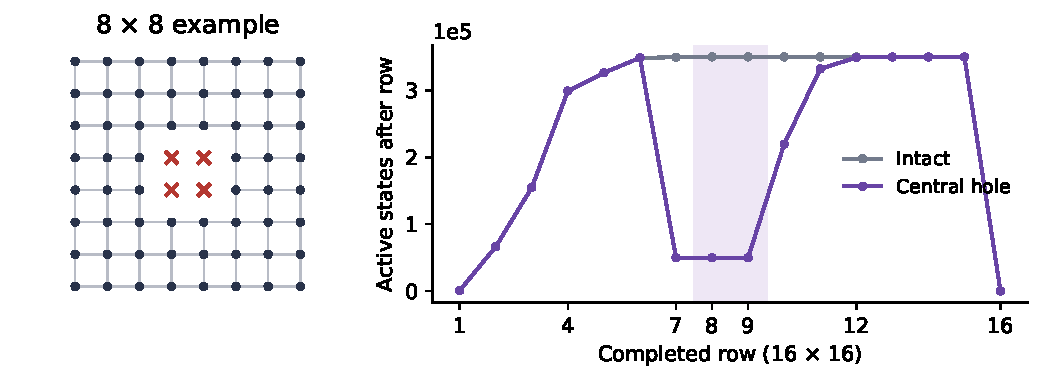
\includegraphics[width=\linewidth]{hole-and-states.pdf}
\caption{Deleted vertices in the $8\times8$ example, and row-end state
counts at side $16$. Shading marks the rows with deleted vertices. The
reduction starts one row earlier because edges into the hole are disabled.
The maximum over all vertex transitions exceeds the row-end maximum.}
\label{fig:states}
\end{figure}

\begin{table}[htbp]
\centering\small
\begin{tabular}{rrrrr}
\toprule
$2n$ & Hole peak & Intact peak & Seconds & RSS (MiB) \\
\midrule
4 & 1 & 11 & 0.000010 & 1.719 \\
6 & 40 & 59 & 0.000040 & 1.750 \\
8 & 339 & 341 & 0.000233 & 1.891 \\
10 & 2,120 & 2,120 & 0.002916 & 2.578 \\
12 & 13,943 & 13,943 & 0.035642 & 5.422 \\
14 & 95,660 & 95,660 & 0.476549 & 24.375 \\
16 & 677,909 & 677,909 & 11.006828 & 315.797 \\
18 & 4,928,252 & 4,928,252 & 19.928776 & 1233.266 \\
20 & 36,572,939 & 36,572,939 & 205.434662 & 9856.422 \\
\bottomrule
\end{tabular}

\caption{Primary-counter peak states for punctured and intact boards. Time and
memory refer to punctured boards. Sides through $16$ use standard hash
maps; larger sides use Boost flat maps, so timings are not directly comparable.}
\label{tab:metrics}
\end{table}

At side $16$, the peak of \PeakStates{} active states first occurs after
row $13$, column $13$. The row-end maximum is $349998$. The two hash maps
coexist during a transition; process RSS includes both maps, their buckets,
and allocator overhead. The recorded run took \RunSeconds{} seconds and
used \PeakMemory{} MiB peak RSS.
Measurements are single observations on an Apple M4 Max with $128$~GiB RAM,
using Apple clang 21.0.0 with \texttt{-O3 -std=c++17}. They are not repeated,
isolated performance benchmarks. The larger runs use
Boost 1.92.0 flat hash maps for aggregation. The explicit-partner counter
also supports local updates to partner fields rather than decoding and
re-encoding the whole frontier at every vertex. These changes preserve the
state definition and recurrence. All $46$ established raw and symmetry
runs were rechecked with the flat-map backend, including peak states.
The punctured side-$18$ count was also checked with both original
standard-map implementations. Some extension and validation runs overlapped
on the workstation; their timings are not isolated comparisons.

Pruning uses degree constraints, missing-neighbor constraints, and rejection
of premature cycles. The raw counter does not identify states under
rotations or reflections, and does not perform future-reachability pruning.
Symmetries are counted separately by the reductions below.

\section{Fixed cycles on smaller boards}
Write $R_2$ for the number of full-board cycles fixed by $180^\circ$ rotation,
$R_4$ for those fixed by $90^\circ$ rotation, $F$ for those fixed by one
specified axial reflection, and $B$ for those fixed by both axial
reflections. These counts depend on $n$, suppressed in the notation.
The symmetry counter uses explicit endpoint partners and temporary boundary
stubs, and never closes a path inside the smaller board.

\subsection{Half board: \texorpdfstring{$F$ and $R_2$}{F and R2}}
Take rows $1$ through $n$, with the two central vertices deleted from the
last row. A reflection-fixed spanning cycle must cross the reflection axis.
Every crossing edge is fixed setwise. The induced order-two cycle
automorphism is either a reflection or a half-shift. A half-shift fixes no
edge setwise, so the crossing rules it out. Thus the automorphism is a
reflection with no fixed vertices and exactly two fixed edges. These are
exactly the two crossings. The retained half is a Hamiltonian path with both endpoints
at allowed positions on the cut. Counting final states with exactly two
paired stubs gives $F$.

The half-turn has its center at a lattice face center and fixes no vertex
or edge setwise. It therefore acts freely on vertices and edges of the
cycle. Identify omitted vertices with their rotated representatives.
On the cut, pair column $x$ with column $2n+1-x$. Selected seam edges complete
the half-board paths into a quotient cycle. Require one quotient component
and an odd number of seam edges. Each seam changes the copy index by one
modulo two, so odd parity makes the lift one cycle instead of two.
This gives $R_2$ without constructing full-board cycles.

\subsection{Quarter board: \texorpdfstring{$R_4$ and $B$}{R4 and B}}
For a quarter-turn, use the $n\times n$ quadrant with corner $(n,n)$ deleted.
Add seam edges joining $(n,k)$ to $(k,n)$, for $1\leq k<n$.
A connected quotient cycle lifts to one cycle on four copies precisely when
its net change of copy index is coprime to four. Each seam contributes
$+1$ or $-1$. Thus the condition is equivalent to an odd number of seam edges.
Final states are tested for this parity and a single quotient component.
This is the punctured analogue of the quadrant construction used by
Wynn~\cite{wynn} for intact grids.

\begin{figure}[htbp]
\centering
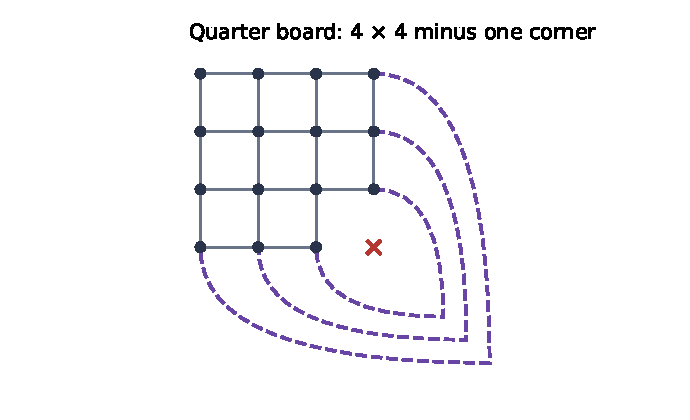
\includegraphics[width=.58\linewidth]{quarter-quotient.pdf}
\caption{Quarter-board quotient for side $8$. Dashed curves are additional
seam edges, not original grid edges. The corner $(4,4)$ is deleted.}
\label{fig:quarter}
\end{figure}

If a full cycle is fixed by both axial reflections, it crosses each axis
exactly twice. Cutting at those four edges leaves one spanning path in each
quadrant. Its endpoints lie on the two inner sides. Counting quarter-board
states with exactly two paired stubs, one on each inner side, gives $B$.
Reflection reconstructs the full cycle uniquely.

\section{Parity, diagonal reflections, and Burnside's lemma}
\label{sec:burnside}
\begin{proposition}\label{prop:parity}
If $n\geq3$ is odd, then $G_n$ has no Hamiltonian cycle fixed by a
quarter-turn. Equivalently, $R_4=0$ for odd $n$.
\end{proposition}
\begin{proof}
Color $(x,y)$ by the parity of $x+y$. A quarter-turn sends it to
$(2n+1-y,x)$ and exchanges the colors. Suppose a Hamiltonian cycle $C$
is fixed by this rotation. Its length is $N=4n^2-4$.
The induced automorphism of $C$ has order four, since $C$ spans the graph
and the quarter-turn acts faithfully on its vertices. Every order-four
automorphism of an undirected cycle is a cyclic shift by $N/4$ or $3N/4$
positions. These are $n^2-1$ and $3(n^2-1)$ positions. If $n$ is odd,
both shifts are even. Since colors alternate around $C$, such a shift
preserves color, contradicting the color exchange of the quarter-turn.
\end{proof}
The empty case $n=1$ also has $R_4=0$ by convention. The deletion reverses
the corresponding parity obstruction for intact grids~\cite{wynn}.

\begin{samepage}
\begin{proposition}\label{prop:diagonal}
For $n\geq3$, neither diagonal reflection fixes a Hamiltonian cycle of $G_n$.
\end{proposition}
\begin{proof}
Each diagonal reflection fixes $2n-2\geq4$ remaining vertices. If it
preserved a Hamiltonian cycle, its restriction would be a nonidentity
cycle automorphism with at least four fixed vertices. A nonidentity cycle
automorphism fixes at most two vertices, a contradiction.
\end{proof}
\end{samepage}

Let $O_n$ count geometric orbits of Hamiltonian-cycle edge sets under $D_4$.
For $n\geq3$, Proposition~\ref{prop:diagonal} and Burnside's lemma give
\begin{equation}\label{eq:burnside}
O_n=\frac{H_n+R_2+2R_4+2F}{8}.
\end{equation}
The two quarter-turns have the same fixed set, and the two axial reflections
are conjugate. For $n=2$, add the two diagonal-reflection contributions of
one before dividing by eight; the unique $12$-cycle is fixed by all of $D_4$.
Set $O_1=0$.

\begin{table}[htbp]
\centering\footnotesize
\setlength{\tabcolsep}{4pt}
\begin{tabular}{rrrrr}
\toprule
$n$ & $R_2$ & $R_4$ & $F$ & $B$ \\
\midrule
2 & 1 & 1 & 1 & 1 \\
3 & 2 & 0 & 4 & 2 \\
4 & 398 & 18 & 436 & 20 \\
5 & 39598 & 0 & 58198 & 138 \\
6 & 155368312 & 8650 & 96650662 & 6406 \\
7 & 480564699890 & 0 & 308860488706 & 201338 \\
8 & 34116385160498522 & 106253220 & 10202488985967222 & 41184930 \\
9 & 2811552194264884895872 & 0 & 740001412241179546444 & 6067605252 \\
10 & 3914442037913372967313267520 & 31064776598948 & 515530816787170934773269074 & 5594443405532 \\
\bottomrule
\end{tabular}

\caption{Fixed edge-set counts for the punctured grids. $F$ refers to one
specified axial reflection; $B$ requires both.}
\label{tab:fixed}
\end{table}
\begin{table}[htbp]
\centering\small
\begin{tabular}{rr}
\toprule
$n$ & $O_n$ \\
\midrule
1 & 0 \\
2 & 1 \\
3 & 3 \\
4 & 20676 \\
5 & 1210546548 \\
6 & 3483478580414922 \\
7 & 145938676601947358766460 \\
8 & 189627697916042276889063633686282 \\
9 & 4450608400247986041886906383605585167240715 \\
10 & 2774300066395485992532938392421228045172137752081602347 \\
\bottomrule
\end{tabular}

\caption{Geometric orbits under all eight symmetries of the square.}
\label{tab:orbits}
\end{table}
In particular,
\[
O_8=\OrbitSixteen.
\]
These are geometric equivalence classes, not classes under arbitrary
abstract graph isomorphism. Every computed Burnside numerator is divisible
by eight. This is a consistency check; the separate small-case edge-orbit
search provides a different enumeration check.

\section{Exact stabilizer classes}
For $n\geq3$, a cycle cannot have both quarter-turn and axial-reflection
symmetry, since these would generate a forbidden diagonal reflection.
The five possible exact stabilizers have the orbit counts in
Table~\ref{tab:classformulas}.
\begin{table}[htbp]
\centering\small
\begin{tabular}{lcr}
\toprule
Exact stabilizer & Orbit size & Number of orbits\\
\midrule
Identity only & 8 & $(H_n-R_2-2F+2B)/8$\\
One axial reflection & 4 & $(F-B)/2$\\
Half-turn only & 4 & $(R_2-R_4-B)/4$\\
Both axes and half-turn & 2 & $B/2$\\
Quarter-turn rotations & 2 & $R_4/2$\\
\bottomrule
\end{tabular}
\caption{Exact stabilizer decomposition for $n\geq3$.}
\label{tab:classformulas}
\end{table}

To derive these formulas, first note that $B$ and $R_4$ count disjoint sets
with order-four stabilizers, each with two members per orbit. Subtracting
these sets from $R_2$ leaves the half-turn-only edge sets in orbits of size
four. Each one-reflection orbit has two members fixed by the specified axis,
which gives $(F-B)/2$. Subtracting all nontrivial stabilizers from $H_n$
gives the identity-only count. This bookkeeping follows the corresponding
intact-grid analysis of Wynn~\cite{wynn}.

\begin{table}[htbp]
\centering\small
\begin{tabular}{lr}
\toprule
Exact stabilizer & Number of orbits \\
\midrule
Identity only & 189627697916042263258722834310968 \\
One axial reflection & 5101244472391146 \\
$180^\circ$ rotation only & 8529096253265093 \\
Both axial reflections & 20592465 \\
Quarter-turn rotations & 53126610 \\
Full $D_4$ & 0 \\
Total & 189627697916042276889063633686282 \\
\bottomrule
\end{tabular}

\caption{Exact symmetry classes for the $16\times16$ punctured grid.}
\label{tab:classes}
\end{table}
The class counts are nonnegative integers at every computed size. Their sum
is $O_n$, and weighting them by the orbit sizes $8,4,4,2,2$ recovers $H_n$.
For $n=2$, there is instead one orbit with full $D_4$ stabilizer and orbit
size one.

\section{Finite-size comparison with intact grids}
Let $C_n$ count undirected Hamiltonian cycles on the intact $2n\times2n$
grid, as in OEIS A003763~\cite{oeis}. Both full counters reproduce its
values for $n\leq\MaximumN$; the OEIS b-file contains terms through $n=13$. Define
\[
Q_n=\frac{H_n}{C_n},\qquad
c_n=C_n^{1/(4n^2)},\qquad h_n=H_n^{1/(4n^2-4)}.
\]
The same-footprint ratio $Q_n$ is not a probability of surviving vertex
deletion: deleting vertices from an intact Hamiltonian cycle generally
does not leave a Hamiltonian cycle. The per-vertex quantities $c_n$ and
$h_n$ are finite-size growth estimators. Both vertex count and boundary
corrections matter in interpreting them.

For context, Jacobsen~\cite[Eq.~(4.5)]{jacobsen} reports the numerical
estimate $\mu=1.472801\pm0.00001$ for the square-lattice Hamiltonian-walk
connective constant, attributing it to Jacobsen and Kondev; his own
circuit-and-walk analysis gives $1.473\pm0.001$ in Eq.~(4.4).
This is a numerical benchmark, not an exact constant or a proven limit
for the punctured sequence considered here.

\begin{table}[htbp]
\centering\small
\begin{tabular}{rrrrr}
\toprule
$n$ & $H_n/C_n$ & $\log Q_n$ & $c_n$ & $h_n$ \\
\midrule
3 & 0.013059701 & -4.338224012 & 1.213869718 & 1.085966682 \\
4 & 0.035377668 & -3.341674516 & 1.271048904 & 1.221570580 \\
5 & 0.020725521 & -3.876389441 & 1.308264601 & 1.270637022 \\
6 & 0.025894009 & -3.653743666 & 1.334201899 & 1.310584485 \\
7 & 0.020801394 & -3.872735292 & 1.353235262 & 1.334597523 \\
8 & 0.023026163 & -3.771124175 & 1.367762905 & 1.354161936 \\
9 & 0.020534244 & -3.885661351 & 1.379198061 & 1.368038963 \\
10 & 0.021749399 & -3.828169175 & 1.388423611 & 1.379631942 \\
\bottomrule
\end{tabular}

\caption{Finite-size ratios and per-vertex growth estimators.}
\label{tab:growth}
\end{table}
\begin{figure}[htbp]
\centering
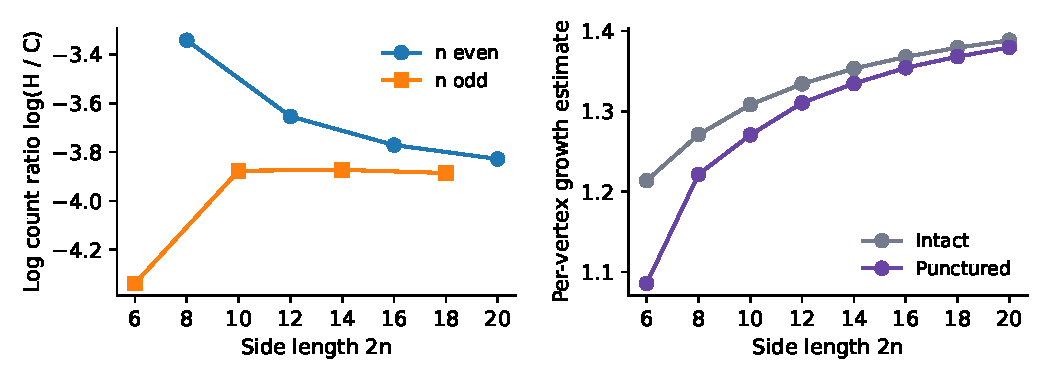
\includegraphics[width=\linewidth]{finite-size.pdf}
\caption{Exact-count comparisons. Lines connect computed values only;
no asymptotic curve is fitted.}
\label{fig:growth}
\end{figure}
Over $3\leq n\leq8$, the even-$n$ ratios decrease and the odd-$n$
ratios increase. The extension to $n=9$ reverses the latter trend:
$Q_9\approx0.020534244$, below $Q_7\approx0.020801394$.
Thus monotone convergence of the odd subsequence is not supported even
by this modest extension. The hole deletes two vertices of each
checkerboard color for every $n$, so color imbalance alone cannot explain
the parity split. At $n=8$, the punctured count is about $2.3026\%$ of the
intact count for the same outer board. The available finite-size values
do not identify an asymptotic exponent or distinguish a constant
prefactor from a slowly changing correction.
The log ratio $\log Q_n$ measures the change in the logarithm of the
number of configurations caused by the defect. Its negative can be viewed
as a dimensionless defect free-energy cost. This observable removes the
common outer footprint without introducing different per-vertex
normalizations. Figure~\ref{fig:growth} plots $\log Q_n$ separately by
parity. Multiplying $Q_n$ by the numerical benchmark $\mu^4$ would
compensate heuristically for four missing vertices; on the log scale this
only adds $4\log\mu$. It does not establish a limiting defect cost.
A constant limit, logarithmic correction, and parity-dependent corrections
remain hypotheses to test with larger boards. No gluing argument proving
equality of the bulk coefficients is supplied here.

\section{Reproducibility and related work}
\label{sec:reproducibility}
The public repository
\url{https://github.com/jroell/punctured-grid-cycles}
contains the source code, recorded data, and manuscript build instructions.
The complete exact-count reference is commit
\href{https://github.com/jroell/punctured-grid-cycles/tree/2d0d15baa21d21f9436bcf5736be4969a0ad818f}{\texttt{2d0d15b}}.

\subsection{Verification}
The parenthesis and direct-partner frontier counters agree on all intact
and punctured boards at every even side from $2$ through $\MaximumSide$.
They share the integer type and the row-by-row decomposition, so these are
separately encoded cross-checks, not wholly independent mathematical
methods. Direct path enumeration checks the complete cycle sets at
punctured sides $4$ and $6$, including all eight symmetry actions.
A different Python checker branches on whole edge orbits and independently
verifies $R_2,R_4,F,B$ through punctured side $8$. Additional runs of
that checker verify $R_4$ and $B$ at sides $10$ and $12$. Larger fixed-set
counts still rely on the quotient implementation and consistency checks,
not an independent second enumeration.
The intact results agree with OEIS A003763~\cite{oeis}.

From a repository checkout, run
\begin{verbatim}
make all
make benchmark
make test
make flat BOOST_CPPFLAGS=-I/opt/homebrew/include
python3 scripts/verify_backends.py
python3 scripts/verify_more_symmetry.py
python3 scripts/extend.py --backend flat
python3 scripts/extend_symmetry.py
python3 scripts/verify_extension.py
uv sync --group paper
uv run --group paper python scripts/build_paper.py
\end{verbatim}
The optional Boost include path shown is for Homebrew on Apple Silicon;
omit it when Boost headers are on the default compiler include path.
The counters need a C++17 compiler supporting \texttt{unsigned \_\_int128}
and Python 3.11 or later. The manuscript build additionally uses Tectonic
and Pandoc; the Python document dependencies are pinned in \texttt{uv.lock}.
The original full-board benchmark uses a $300$-second timeout per run. The symmetry counter
stops after $1800$ seconds or fifty million active states. The original
symmetry benchmark additionally has a $260$-second subprocess timeout.
Larger raw runs have a $1800$-second timeout and a monitored $48$~GiB
RSS ceiling; the RSS monitor polls every two seconds. Each small
edge-orbit check has a $60$-second limit. All jobs run finite case lists.
Counts are stored as decimal strings in JSON to avoid floating-point
rounding. Timings and memory use may differ by platform.

\subsection{Prior work and scope}
Wynn~\cite{wynn} counts symmetry classes for intact square grids and uses
quadrant quotients for quarter-turn symmetry. Jacobsen~\cite{jacobsen}
enumerates circuits, walks, and chains by transfer methods.
Blanco and Zeilberger~\cite{blanco} give a recent fixed-width
generating-function implementation. The present note applies these ideas
to a specified central puncture and records a reproducible table through
side $\MaximumSide$.

OEIS searches for consecutive terms of both $H_n$ and $O_n$ returned no
match on September 26, 2026. These searches and the literature check are
not exhaustive and do not establish priority. No OEIS identifier or
preprint identifier is asserted before it has been assigned.

\begin{thebibliography}{9}
\bibitem{oeis}
OEIS Foundation Inc., \emph{The On-Line Encyclopedia of Integer Sequences},
entry \href{https://oeis.org/A003763}{A003763}, accessed September 26, 2026.
\bibitem{wynn}
E. Wynn, Enumeration of nonisomorphic Hamiltonian cycles on square grid
graphs, preprint, 2014, \href{https://arxiv.org/abs/1402.0545}{arXiv:1402.0545}.
\bibitem{jacobsen}
J. L. Jacobsen, Exact enumeration of Hamiltonian circuits, walks, and chains
in two and three dimensions, \emph{J. Phys. A: Math. Theor.}
\textbf{40} (2007), 14667--14678.
\href{https://doi.org/10.1088/1751-8113/40/49/003}{doi:10.1088/1751-8113/40/49/003}.
\bibitem{blanco}
P. Blanco and D. Zeilberger, Counting (and randomly generating) Hamiltonian
cycles in rectangular grids, preprint, 2026,
\href{https://arxiv.org/abs/2603.24315}{arXiv:2603.24315}.
\end{thebibliography}
\end{document}
